Energy-aware task coalescing strategies gain \sys efficiency, and the flexible time-based task splitting strategy enables \sys to progress where its counterparts fail.

\subsection{Task Coalescing}
\label{sec:task_coalescing}

% \begin{wrapfigure}{t!}{0.5\textwidth}
% 	\centering
% 	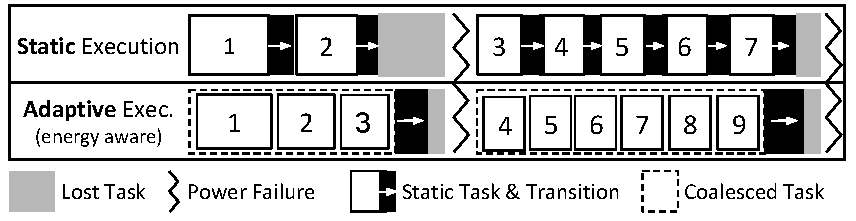
\includegraphics[width=0.5\columnwidth]{figures/coal_Intro_Figure.pdf}
% 	\caption{When $N$ tasks coalesced $N-1$ commit operations are skipped.}
% 	\label{fig:coalIntro}
% \end{wrapfigure}

\noindent When incoming energy is sufficient to run multiple consecutive tasks,
committing state after each task is wasteful. \sys mitigates this
waste by deferring the expensive commits and performing them in a
batch. In the resulting execution, several tasks are \emph{merged} into a
single virtual task---a process we call \emph{coalescing}. 


\noindent When $N$ tasks are coalesced, $N-1$ boundaries are crossed and some number of
pages are dirtied. The first $N-2$ executions of \transition statement skip
committing dirty pages to non-volatile memory, leaving the work of committing
pages modified by any of the $N$ tasks to the statement $N-1$.Therefore, coalescing static tasks is a twofold benefit: (i) it reduces the total number of non-volatile memory
accesses when variables are accessed many times within a coalesced task and committed only conly at the coalesced task boundery; (ii) it fasten applicaiton exeution be skipping unnecessary data commits operations when there is abandond energy. 

\textcolor{red}{maybe is possible to demonstrate with data? count number of executed non-volatile vs volatile accesses}
%

\noindent \textbf{Trade-off between Speed and Wasted Effort.} \sys can coalesce an
arbitrary number of consecutive tasks. However, as more tasks coalesce, their
collective commit overhead amortizes better, but the risk of wasting work also
increases. If power fails during a long sequence of coalesced tasks, execution
will restart from the last commit, i.e. the first task in the sequence, losing
the progress made by any of the coalesced tasks. Therefore, a good coalescing strategy must moderate the risk of wasted work and capitalize on benefits of deferred commits by adapting the target size of the dynamic task
to the energy available at runtime. 
%

\noindent \textbf{Task Coalescing Strategies.} 
% % Carlo pseudo code 
% \begin{algorithm}[t]
% 	\caption{Coalescing}
% 	\label{algo:genCoalescing}
% 	\scriptsize
% 	%\small
% 	\begin{algorithmic}[1]
%         \State $H_\text{p} \gets H_\text{c}$
%         \State $H_\text{p} \gets 0$ 
%         \State $B \leftarrow $ \Call{$f_\text{reboot}$}{$B, H_\text{p}$}

%         \While{$\texttt{true}$}
% 	        \State $ B_\text{c} \gets B$
% 	        %
% 	        \While{$ B_\text{c} > 0$}
% 		        \State \Call{execute\_task}{$T_\texttt{i}$}
% 		        \State $W \leftarrow $ \Call{$f_\text{weight}$}{$T_\text{i}$}
% 		        \State $B_\text{c} \gets B_\text{c} - W$
% 				\State $H_\text{c} \gets H_\text{c} + W$
% 	        \EndWhile
% 	        %
% 	         \State $B \leftarrow $ \Call{$f_\text{compl}$}{B, $H_\text{c}$,$H_\text{p}$}
% 	        \State \Call{commit\_to\_fram}{\null}
%         \EndWhile
% 	\end{algorithmic}
% \end{algorithm}
% %
% To describe the proposed strategies we will use the following parameters:
% \begin{itemize}
% \item target budget $B$: total number of static tasks to be coalesced.
% \item current budget $B_\text{c}$: remaining number of tasks to be coalesced before committing to non-volatile memory; 
% \item history $H$: up on reboot, it is the number of executed static tasks between the last two power interrupts. While executing, it is the number of executed static tasks since the last power interrupt.
% \end{itemize}
%
%
% Modifiying Carlo's pseudo code a little 
\begin{algorithm}[t]
	\caption{Coalescing}
	\label{algo:genCoalescing}
	\scriptsize
	%\small
	\begin{algorithmic}[1]
        \State $B \leftarrow $ \Call{$f_\text{reboot}$}{$H$}
        \State $H \gets 0$ 
        \While{$\texttt{true}$}       
	        \State $ i \gets 0$
	        %
	        \While{$ i <= B$}
		        \State \Call{execute\_task}{$T_\texttt{i}$}
		        \State $W \leftarrow $ \Call{$f_\text{weight}$}{$T_\text{i}$}
		        \State $i \gets i + W$
				\State $H \gets H + W$
	        \EndWhile
	        %
	        \State \Call{commit\_to\_fram}{\null}
	        \State $B \leftarrow $ \Call{$f_\text{coalesc\_task\_maker}$}{$B$}
        \EndWhile
	\end{algorithmic}
\end{algorithm}
%
%
The general structure of the proposed coalescing strategies is summaries in algorithm~\ref{algo:genCoalescing}, where, $B$ (target budget) is total number of static tasks to be coalesced; $T_\text{i}$ is the i-th task being executed; $W_\text{i}$ is weight of $T_\text{i}$; and $H$ (history) is the number of executed static tasks between the last two power interrupts, on a reboot, and it is the number of executed static tasks since the last power interrupt, while executing. Furthermore, we use the following function templates to characterize the proposed coalescing algorithms: $f_\text{reboot}$ which updates the target budget after a reboot. $f_\text{weight}$ which returns the weight of the task and its unit. $f_\text{coalesc\_task\_maker}$ which specifies the size of the coalesced task size. The following sections detail the different strategies \sys proposes and the needs that originated from one strategy leading to the conception of another one.

\subsubsection{Energy-blind Coalescing (EB)}
\label{subsec:energyBlind}

\begin{wrapfigure}{t!}{0.5\textwidth}
	\centering
	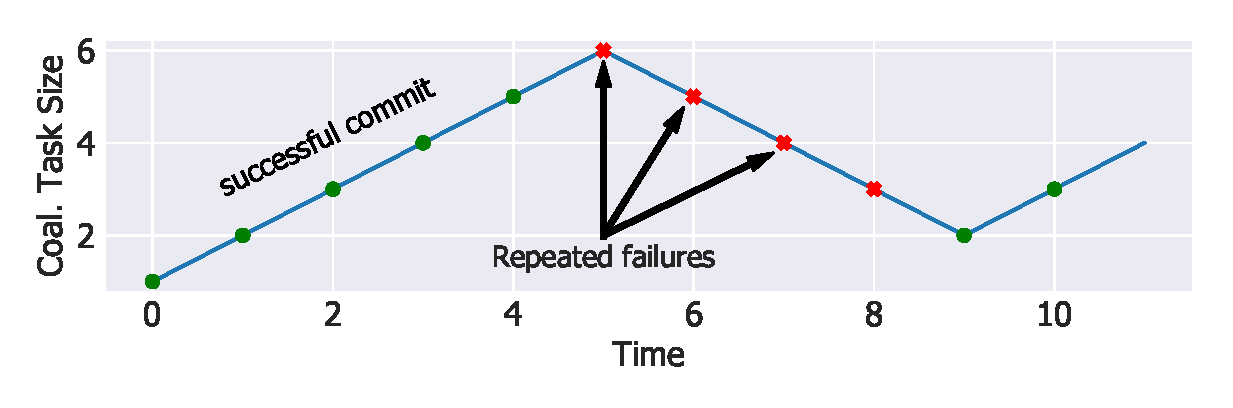
\includegraphics[width=0.5\columnwidth]{figures/slowCoal}
	\caption{The {\em energy blind coalescing} algorithm \emph{linearly} updates its coalescing target.}
	\label{fig:energyBlind}
\end{wrapfigure}

The need for \emph{adaptiveness}, that is coalescing static tasks, can be fulfilled by a naive strategy, having the target budget $B$ to increase by $x$ static tasks after a successful completion of a coalesced task, and to decrease by the same number of tasks upon a reboot. In this case: 
\begin{itemize}
\item $f_\text{reboot}(B) = B - x $;
\item $f_\text{weight}(T_\text{i}) =  1$; 
\item $f_\text{coalesc\_task\_maker}(B) = B + x$; 
\end{itemize}
Since this algorithm relies on an \emph{energy blind counting process} that enlarges the coalesced task size by $x$ static tasks on a successful completion, and reduces its size by $x$ on a reboot. this algorithm is slow in reacting to the changes in energy conditions; the energy required by a coalesced task or the available energy. In particular, this algorithm can experience a large number of \emph{repeated power} failures without forward progress, (see figure~\ref{fig:energyBlind}). In other words, if a coalesced task size is enlarged ten times, due to ample amount of energy or coalescing small static tasks, and then the algorithm can only progress by a single static task, due to a change in energy condition, the device has to reboot for ten times to have an adequate coalesced task size. Moreover, This algorithm tends to experience a large re-execution penalty due to its unawareness of the energy conditions and it optimistic behavior.

\subsubsection{Energy-aware Coalescing (EA)}
\label{subsec:energyAware}
The Energy-aware coalescing algorithm overcomes the limitations of the previous algorithm, with out losing generality or requiring hardware support, by using the recent execution history as a metric---pure software technique---to estimate the available energy and to set the size of the coalescing task accordingly. Moreover, it takes advantage of the guarantees that the energy buffer offers on a fresh start by coalescing many static tasks. Then it approaches the expected power failure carefully by reduces the task target size by x\%, amongst 25\%, 50\% and 75\% the 50\% shows the best performance and therefore it is the default of \sys. if twice the number of the estimated tasks has been executed in the same power discharging cycle the algorithm concludes a wrong power failure time estimation has happened and enforce target re-tuning based on its new history. The EA algorithm is characterized by the following functions: 

\begin{itemize}
\item $f_\text{reboot}(B) = floor(H / 2);$
\item $f_\text{weight}(T_\text{i}) =  W_\text{i}$; 
\item $f_\text{coalesc\_task\_maker}(B) = floor(H / 2);$ 
\end{itemize}

\begin{wrapfigure}{}{0.5\textwidth}
	\centering
	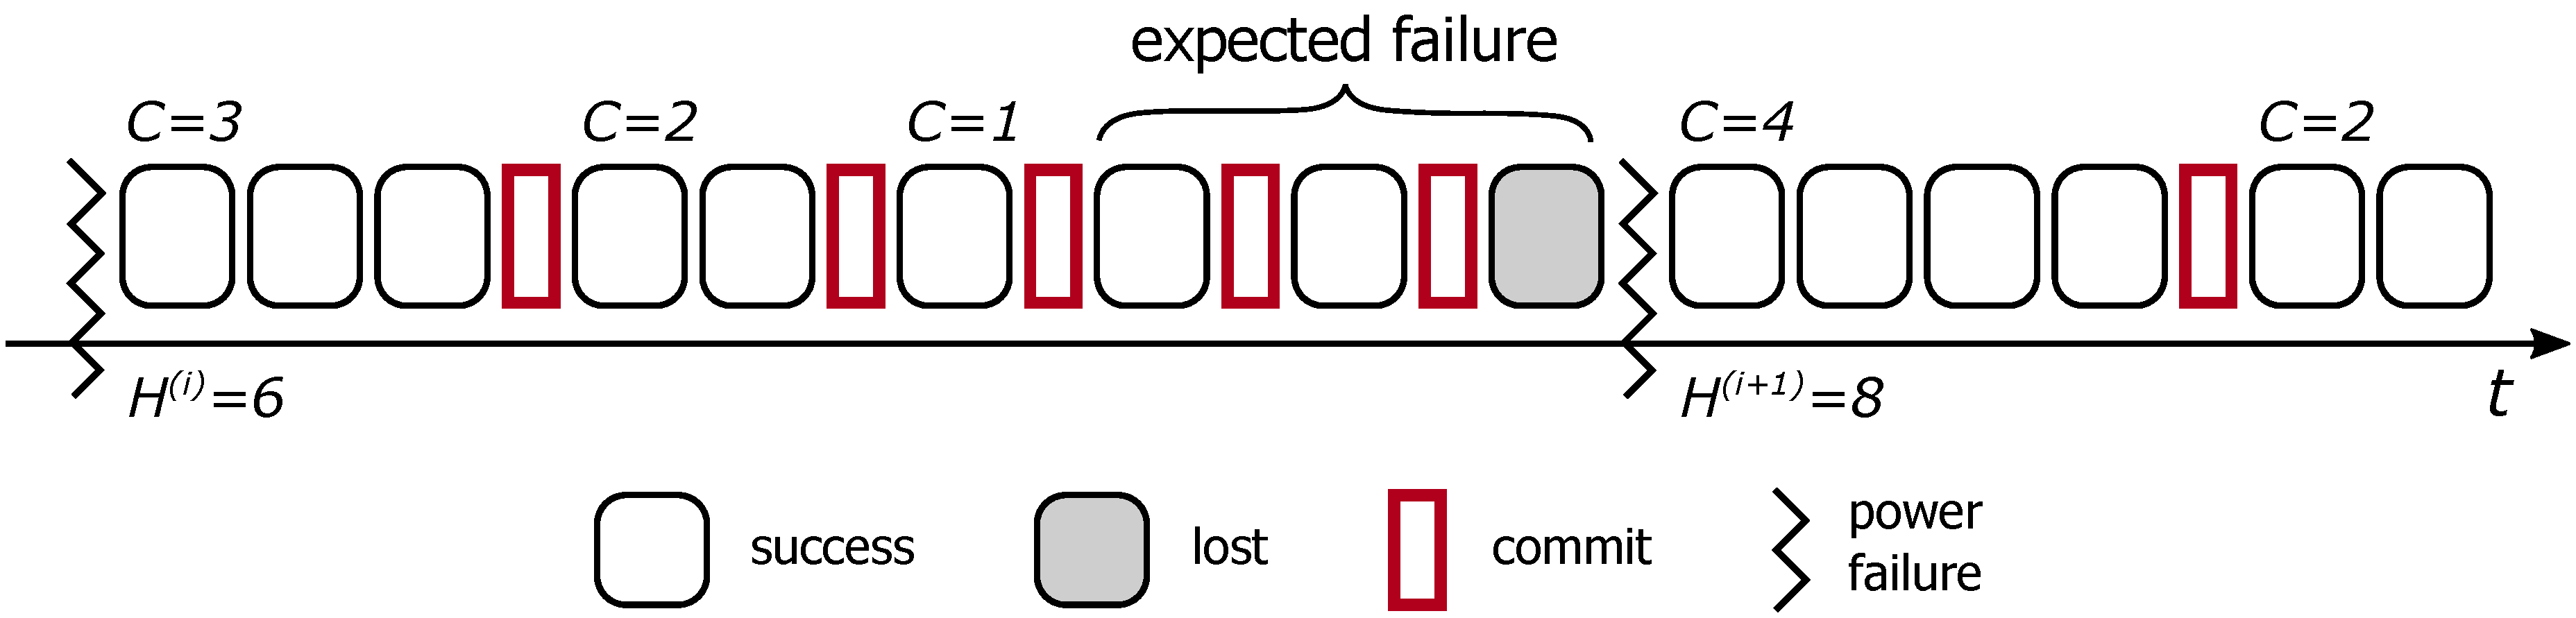
\includegraphics[width=0.5\columnwidth]{figures/energy-aware-coal.pdf}
	\caption{placeholder}
	\label{fig:energyAware}
\end{wrapfigure}


\subsubsection{Energy- and Task-aware Coalescing (EA)}
\label{subsec:energyTaskAware}





























